\documentclass[tikz]{standalone}
\usetikzlibrary{positioning}

\begin{document}
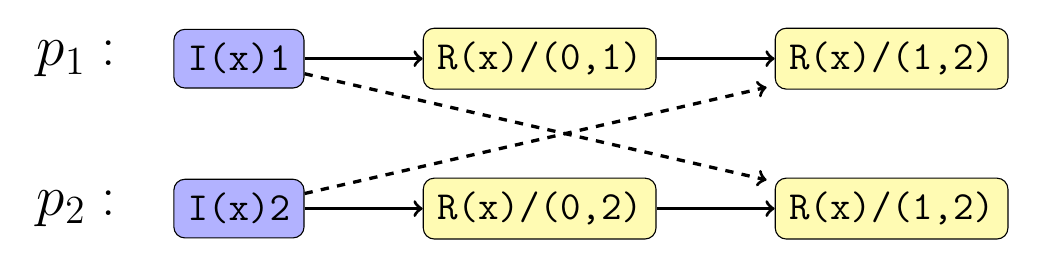
\begin{tikzpicture}
\tikzset{
  wop/.style = {rectangle, rounded corners, fill = blue!30, draw, font = \Large, inner sep = 5pt},
  rop/.style = {rectangle, rounded corners, fill = yellow!30, draw, font = \Large, inner sep = 5pt}, process/.style = {font = \huge}, po/.style = {->, very thick},
  rw/.style = {->, shorten >= 3pt, very thick, dashed},
  vis/.style = {->, shorten >= 3pt, very thick, dashed}
}

  \node (p1) [process] {$p_1:$};
  \node (ix1) [wop, right = 0.6cm of p1] {\texttt{I(x)1}};
  \node (rx1) [rop, right = 1.5cm of ix1] {\texttt{R(x)/(0,1)}};
  \node (p1rx12) [rop, right = 1.5cm of rx1] {\texttt{R(x)/(1,2)}};

  \node (p2) [process, below = 1.2cm of p1] {$p_2:$};
  \node (ix2) [wop, right = 0.6cm of p2] {\texttt{I(x)2}};
  \node (rx2) [rop, right = 1.5cm of ix2] {\texttt{R(x)/(0,2)}};
  \node (p2rx12) [rop, right = 1.5cm of rx2] {\texttt{R(x)/(1,2)}};
  
  \draw [po] (ix1) to (rx1);
  \draw [po] (rx1) to (p1rx12);

  \draw [po] (ix2) to (rx2);
  \draw [po] (rx2) to (p2rx12);
  
  \draw [vis] (ix1) to (p2rx12);
  \draw [vis] (ix2) to (p1rx12);
\end{tikzpicture}
\end{document}
